\section{Dinghy Performance}

Testing the algorithm using the previously defined test.


As we see the small clusters in both algorithms have definitively higher recover times than those of the larger cluster.
While this might seem counterintuitive at first, in a system this isolated and latency free, random timeouts can have larger effects on the quick recover of a cluster.
Probabilistically this makes sense. A cluster will settle on a leader quite quickly after a node has recognized the leader to be down, and if this timeout is based on some random variable, the clusters with more nodes will have a greater probability of getting a smaller timeout that catches the downed leader quicker.
Though with this consideration, we can quickly see the effects that larger cluster size have. The recover time of the cluster sky rocketed when more and more nodes were introduced.
What we also see however is that the test with Dinghy taking consistently less time to recover than pure Raft.

From the generated 99\% confidence intervals, we see that Dinghy consistently, and signficantly out performs pure Raft in terms of fault tolerance and its ability to scale. With this we can confidently say that Dinghy does in fact assist the Raft algorithm in scaling for larger cluster sizes, as the confidence interval for the difference betweent their recover times, does not include 0, which would indicate their equality in performance.


%Table of data

\begin{table*}[t]
	\centering
	\caption*{Time Taken To Recover After Downed Leader Node (ms) with 99\% Confidence}
	\begin{tabular}{|c||c|c|c|c|}
	\hline
 	Cluster Size & Vanilla Raft & Dinghy Raft & Improvement with Dinghy \\ 
  	\hline
	3 & 651.37 & 647.03 & 4.34$\pm$15.10 \\ 
	5 & 588.19 & 591.35 & -3.16$\pm$10.46 \\ 
	7 & 567.63 & 569.95 & -2.32$\pm$8.08 \\ 
	9 & 570.70 & 566.82 & 3.88$\pm$6.60 \\ 
	11 & 567.32 & 565.99 & 1.34$\pm$5.81 \\ 
	13 & 572.61 & 568.80 & 3.81$\pm$5.13 \\ 
	15 & 578.28 & 574.51 & 3.77$\pm$4.45 \\ 
	17 & 585.55 & 579.99 & 5.55$\pm$4.15 \\ 
	19 & 592.69 & 587.49 & 5.21$\pm$3.88 \\ 
	21 & 602.72 & 592.97 & 9.75$\pm$3.52 \\ 
	23 & 608.53 & 603.38 & 5.15$\pm$3.40 \\ 
	25 & 617.42 & 612.26 & 5.16$\pm$3.36 \\ 
	27 & 625.49 & 619.40 & 6.09$\pm$3.15 \\ 
	29 & 635.61 & 629.62 & 5.99$\pm$3.17 \\ 
	31 & 643.91 & 637.29 & 6.62$\pm$3.58 \\ 
	33 & 654.19 & 646.85 & 7.33$\pm$2.96 \\ 
	35 & 666.01 & 658.18 & 7.84$\pm$3.01 \\ 
	37 & 673.07 & 667.24 & 5.83$\pm$2.81 \\ 
	39 & 683.04 & 675.68 & 7.36$\pm$2.86 \\ 
	41 & 694.01 & 684.85 & 9.16$\pm$2.77 \\ 
	43 & 703.16 & 695.15 & 8.01$\pm$2.59 \\ 
	45 & 712.46 & 704.71 & 7.76$\pm$2.54 \\ 
	47 & 724.06 & 714.48 & 9.58$\pm$2.54 \\ 
	49 & 732.84 & 723.64 & 9.20$\pm$2.51 \\ 
	51 & 742.69 & 733.71 & 8.98$\pm$2.55 \\ 
	\hline
	\end{tabular}
\end{table*}


%Graphs of Performance


\begin{figure}[!h]
\centering
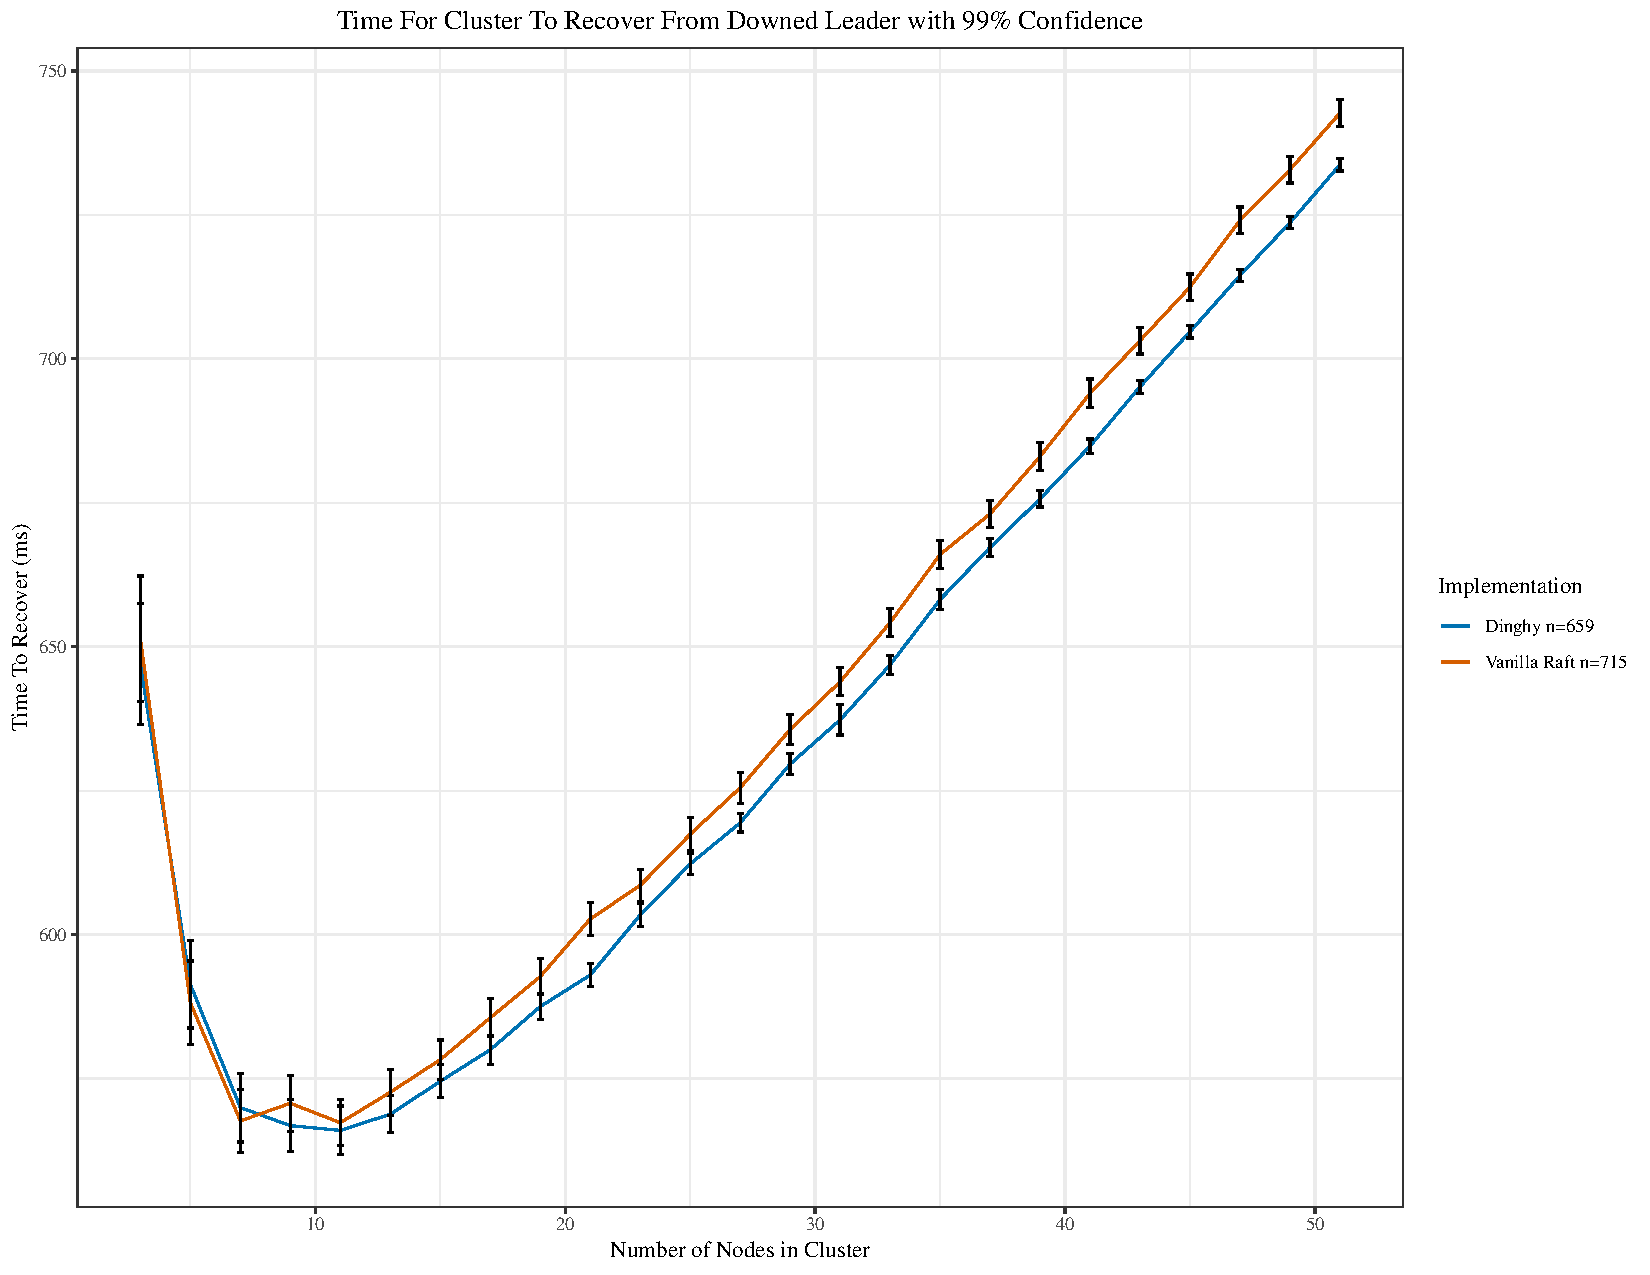
\includegraphics[width=0.5\textwidth]{dinghy.pdf}
\end{figure}


